\documentclass[11pt]{article}
\usepackage[T1]{fontenc}
\usepackage{lmodern}
\usepackage[margin=1.05in]{geometry}
\usepackage{amsmath,amssymb,amsthm,mathtools}
\usepackage{microtype}
\usepackage{enumitem}
\usepackage{booktabs}
\usepackage{tikz}
\usetikzlibrary{arrows.meta,calc}
\usepackage{needspace}
\usepackage[hidelinks]{hyperref}
\usepackage[nameinlink,capitalise,noabbrev]{cleveref}
\newcommand{\R}{\mathbb R}
\newcommand{\eps}{\varepsilon}
\newcommand{\area}{\operatorname{area}}
\newcommand{\vol}{\operatorname{vol}}
\newcommand{\ip}[2]{\langle #1,#2\rangle}
\newcommand{\norm}[1]{\lVert #1\rVert}
\DeclareMathOperator{\tr}{tr}
\DeclareMathOperator{\diam}{diam}
\DeclareMathOperator{\conv}{conv}
\DeclareMathOperator{\dist}{dist}
\newtheorem{theorem}{Theorem}[section]
\newtheorem{lemma}[theorem]{Lemma}
\newtheorem{proposition}[theorem]{Proposition}
\newtheorem{corollary}[theorem]{Corollary}
\theoremstyle{remark}
\newtheorem{remark}[theorem]{Remark}
\numberwithin{equation}{section}
\setlist{itemsep=2pt,topsep=4pt}
\setlength{\emergencystretch}{1.2em}

\hypersetup{
  pdftitle={Finite angular cylinder covers below the half-area bound},
  pdfauthor={OpenAI},
  pdfsubject={Mathematics manuscript dated September 27, 2026}
}
\title{Finite angular cylinder covers\\below the half-area bound}
\author{OpenAI}
\date{September 27, 2026}
\begin{document}
\maketitle
\begin{abstract}
A regular tetrahedron admits a finite cylinder covering with compact triangular
perpendicular bases whose total area is less than half its minimum orthogonal
projection area. This disproves the half-area cylinder-covering conjecture.
By affine invariance, the same construction gives a counterexample to the
directionwise normalized half-bound for every nondegenerate tetrahedron.
\end{abstract}
\section{Introduction}

How small can the total cross-sectional area of a finite cylinder covering
of a convex body be? Here a convex body $K\subset\R^3$ is compact, convex,
and has nonempty interior. A cylinder is a set
\[
 C=B+\R u,
\]
where $u$ is a unit vector and its base $B\subset u^\perp$ is measurable
with finite area. All areas and projections are Euclidean. Write
\[
 A_{\min}(K)=\min_{\dim E=2}|\pi_EK|,
\]
where $\pi_E$ is orthogonal projection onto the two-dimensional linear
subspace $E$ and $|\cdot|$ denotes planar Lebesgue measure.
The \emph{half-area cylinder covering conjecture} asks whether every
finite covering $K\subset\bigcup_{i=1}^m(B_i+\R u_i)$ satisfies
\begin{equation}\label{eq:conjectured-bound}
 \sum_{i=1}^m|B_i|\ge\tfrac12 A_{\min}(K).
\end{equation}

The cylinder question belongs to the line of covering problems that begins
with Tarski's plank problem. A \emph{plank} is the region between two
parallel hyperplanes, and its width is their distance. Bang proved that
a finite plank covering of a convex body has total width at least the
body's minimum width~\cite{Bang1951}; see also
\cite[Theorem~2.1]{Bezdek2009}.
Ball proved the directionwise refinement for centrally symmetric bodies:
after dividing each plank's width by the body's width in the same normal
direction, the sum is at least one~\cite[arXiv v1, Theorem~1]{Ball1991}.
Thus the width cost of a plank cover has both an absolute formulation
and a relative formulation adapted to the individual directions.

For cylinders in three dimensions, the two-cylinder cover of a regular
tetrahedron shows that replacing widths by base areas cannot preserve
the constant one. Its two axes are parallel to opposite edges, and its
total base area equals half the tetrahedron's minimum projection area.
Bezdek~\cite[Problem~3.1]{Bezdek2009} and
Bezdek and Litvak~\cite[arXiv v1, Introduction]{BL2009} attribute this example and
the resulting half-area question to Bang's 1951 paper. Their formulations
allow measurable bases perpendicular to the axes, as in our definition.

For a finite covering $\mathcal C=(B_i+\R u_i)_{i=1}^m$, define the
\emph{directionwise relative area} by
\begin{equation}\label{eq:relative-cost}
 \mathcal R(\mathcal C;K):=
 \sum_{i=1}^m\frac{|B_i|}{|\pi_{u_i^\perp}K|}.
\end{equation}
All denominators are positive because $K$ has nonempty interior.
Bezdek and Litvak proved $\mathcal R(\mathcal C;K)\ge1/3$
for every finite covering in three dimensions, and the stronger bound
$\mathcal R(\mathcal C;K)\ge1$ when $K$ is an
ellipsoid. In their proof, the general case combines the Rogers--Shephard
section--projection inequality with a volume comparison. For ellipsoids,
they reduce to a ball and use a density whose integral along every
interior chord is the same~\cite[arXiv v1, Theorem~3.1 and its proof]{BL2009}.
These arguments leave
a gap between the universal one-third lower bound and the proposed
one-half threshold.

Bezdek and Khan record the directionwise assertion
$\mathcal R(\mathcal C;K)\ge1/2$ under the name
\emph{1-Codimensional Cylinder Covering Conjecture}
\cite[arXiv v2, Definition~3 and Conjecture~4.13]{BK2016}.
It would imply \eqref{eq:conjectured-bound}, since
\begin{equation}\label{eq:cost-comparison}
 \mathcal R(\mathcal C;K)
 \le \frac{\sum_i|B_i|}{A_{\min}(K)}.
\end{equation}
Verreault's 2026 survey records the half-area question as
unresolved~\cite[Question~4.14]{Verreault2026}.
Our construction starts with the tetrahedral equality example itself
and replaces its two axes by finitely many nearby directions. It
violates both half-area bounds while retaining compact triangular bases.


We construct a counterexample with compact triangular bases. Set
$H=\sqrt2$ and
\begin{equation}\label{eq:tetrahedron}
 K=\{(x,y,Ht):0\le t\le1,\ |x|\le1-t,\ |y|\le t\}.
\end{equation}
Its vertices are $(\pm1,0,0)$ and $(0,\pm1,H)$, so it is a regular
tetrahedron of edge length $2$.

\begin{theorem}\label{thm:counterexample}
The tetrahedron \eqref{eq:tetrahedron} has $A_{\min}(K)=\sqrt2$.
For every $0<\eps\le1/2000$, it admits a covering by
$m=2\lceil2/\eps^2\rceil$ cylinders with compact triangular perpendicular
bases such that
\begin{equation}\label{eq:main-asymptotic}
 \frac1{\sqrt2}\sum_{i=1}^m|B_i|
 =\frac12-\frac{13}{6000}\eps^2+O(\eps^4).
\end{equation}
The remainder has absolute value at most $2\eps^4$, and the total base
area is strictly less than $A_{\min}(K)/2$.
\end{theorem}

Every covering in the theorem is finite, although its number of cylinders
increases as the tilt decreases. Similarities preserve the ratio of base
area to minimum projection area, so the construction applies to every
regular tetrahedron.

\begin{corollary}\label{cor:normalized-covering}
Every nondegenerate tetrahedron $T\subset\R^3$ admits a finite cylinder
covering with compact triangular perpendicular bases for which
\[
 \sum_{i=1}^m\frac{|B_i|}{|\pi_{u_i^\perp}T|}<\frac12.
\]
Thus the 1-Codimensional Cylinder Covering Conjecture is false.
\end{corollary}
\begin{proof}
For the regular tetrahedron $K$, each denominator is at least
$A_{\min}(K)>0$, so the sum is at most
$\sum_i|B_i|/A_{\min}(K)<1/2$ by
Theorem~\ref{thm:counterexample} with $\eps=1/2000$.

The directionwise ratios are invariant under invertible affine
maps~\cite[arXiv v1, Section~3]{BL2009}.
To see this directly, let $A$ be an invertible linear map and set
$v=Au/|Au|$. The linear map
\[
 L=\left.\pi_{v^\perp}A\right|_{u^\perp}:u^\perp\longrightarrow v^\perp
\]
is an isomorphism: $Lb=0$ implies that $Ab$ is parallel to $Au$,
hence $b$ is parallel to $u$, and therefore $b=0$.
The transformed cylinder has perpendicular base $LB$, and
$\pi_{v^\perp}(AK)=L(\pi_{u^\perp}K)$. Both areas are multiplied by
the same positive factor $|\det L|$, so their ratio is unchanged.
Translations also preserve it. Every nondegenerate tetrahedron is an
affine image of $K$; the images of its covering retain the same finite
count and compact nondegenerate triangular bases.
\end{proof}

This affine argument concerns the directionwise ratios. The conclusion
of Theorem~\ref{thm:counterexample}, which uses one minimum projection
area for all directions, is asserted here for regular tetrahedra.

\paragraph{Idea of the proof.}
Bang's equality example covers the parts $t\le1/2$ and $t\ge1/2$ by
cylinders parallel to the $x$- and $y$-axes, respectively. These axes
are parallel to opposite edges of the tetrahedron, and each base is a
triangle. We
subdivide these triangles into narrow sectors and give each sector its
own tilted axis. Tilting reduces the perpendicular area, but it can also
open gaps between neighboring sectors and between the two families.

Two choices prevent these gaps. First, the axes adjacent to a shared
sector side make the planes containing that side coincide. At a point
$(x,y,Ht)$ of the tetrahedron, these planes specify a finite list of
$y$-coordinates beginning at $-t$ and ending at $t$. Hence some adjacent
pair brackets $y$, even if the list is not ordered. This selects a sector
in the first family; exchanging the roles of $x$ and $y$ does the same
for the second. Second, we increase each sector's radial extent by a
quantity of order $\eps^2$. A gap between the families could occur only
near $t=1/2$. There the radial heights of the two intercepts, measured
from their respective tips, have opposite first-order shifts, $-\eps xy$ and $+\eps xy$, so their sum changes only
to second order. The increases can therefore be chosen small enough
that their area cost is less than the quadratic gain from tilting.

Section~\ref{sec:construction} proves the projection minimum and derives
the finite construction. Section~\ref{sec:coverage} proves exact coverage:
a first-crossing argument chooses angular sectors, and a single radial
budget excludes simultaneous failure of their cutoffs.
Section~\ref{sec:area} computes the perpendicular areas. The angular mesh
has size at most $\eps^2$, which keeps the total approximation error of
order $\eps^4$ even as the number of cylinders grows.

The same mechanism permits more freedom than the first construction
uses. Section~\ref{ext:cap-section} gives a common criterion for
continuous radial profiles, squared-radius cutoffs and bounded Cartesian
apertures, and compares midpoint sampling with endpoint-centred sectors.
Its estimates remain uniform as the partition is refined.
Section~\ref{sec:angular-cubic} then lets the radial margin tend to zero
with the tilt. In the same tetrahedron $K$, its normalized cost is
$1/2-\tau^2/240+(25/2)\tau^3+O(\tau^4)$: one family of constructions
attains the quadratic coefficient approached as the fixed margin tends
to zero. Its cylinders cover for $0<\tau\le1$, whereas the explicit
area bound guarantees strict saving for $0<\tau\le1/4000$.
Appendix~\ref{ext:alternate-estimates} gives complementary direct
proofs for curved caps, and Appendix~\ref{ext:scaling-specializations}
collects the exact counts and formulas under other parameter and scale
choices.

\section{Geometry and the finite construction}\label{sec:construction}

We first fix the area scale against which the covering will be measured.
We then specify every triangle and every axis in the finite covering.
The projection calculation is the facet-area-vector form of Cauchy's
projection formula; see \cite[p.~83, equation~(1)]{Martini1991} for its
projection-body formulation. We include the face-by-face proof for this tetrahedron.

\begin{lemma}\label{lem:projection-minimum}
For the tetrahedron \eqref{eq:tetrahedron}, $A_{\min}(K)=H$.
\end{lemma}
\begin{proof}
The outward face area vectors (unit normal multiplied by face area) are
\[
 (0,\pm H,-1),\qquad (\pm H,0,1).
\]
Indeed, the supporting planes are $\pm Hy-z=0$ and
$\pm Hx+z=H$. The displayed outward normals have length $\sqrt3$,
which is the area of each equilateral face of side length $2$.
For a unit vector $u$, the faces with positive scalar product against $u$ project to partition the shadow, apart from the projections of edges and parallel faces, which have area zero.
They give the forward endpoints of the chords parallel to $u$.
The projected area of a face with area vector $N$ is $|N\cdot u|$,
as follows by projecting its two edge vectors and taking their cross product.
The sum of the four area vectors is zero. Thus the shadow area is half the sum of their absolute scalar products with $u$, namely
\[
 A(u)=\max(H|u_x|,|u_z|)+\max(H|u_y|,|u_z|).
\]
Put $U=\max(|u_x|,|u_z|/H)$ and $V=\max(|u_y|,|u_z|/H)$.
Since $H^2=2$,
\[
 (U+V)^2\ge |u_x|^2+|u_y|^2+2|u_z|^2/H^2=1.
\]
Here $U^2\ge|u_x|^2$, $V^2\ge|u_y|^2$ and
$UV\ge|u_z|^2/H^2$ account for the three terms separately.
Hence $A(u)=H(U+V)\ge H$, with equality at $u=(1,0,0)$.
\end{proof}

At zero tilt, the part $t\le1/2$ is covered by an $x$-parallel cylinder and the part $t\ge1/2$ by a $y$-parallel cylinder.
Each perpendicular base is a triangle of area $H/4$.
The lower intercept triangle can be parametrized as
\[
 (0,qt_0,Ht_0),\qquad -1\le q\le1,\quad 0\le t_0\le1/2.
\]
Here $q$ is a slope parameter: for $t_0>0$ it is the second coordinate
divided by $t_0$.
We call the intervals of $q$ angular sectors. The radial height $t_0$
is the third physical coordinate divided by $H$, rather than Euclidean
distance from the tip. The upper intercept triangle is similarly
$(ps_0,0,H(1-s_0))$, with $-1\le p\le1$ and $0\le s_0\le1/2$.
We now perturb a finite subdivision of these triangles.

Fix a positive tilt parameter $\eps$, and put
\begin{equation}\label{eq:parameters}
 \eta=\frac1{1000},\qquad
 n=\left\lceil\frac2{\eps^2}\right\rceil,\qquad
 \Delta=\frac2n,\qquad q_j=-1+j\Delta\quad(0\le j\le n).
\end{equation}
In particular $\Delta\le\eps^2$.
To make adjacent tilted sectors meet, prescribe the displacement of the
boundary with angular parameter $q$ by
\[
 \phi(q)=\frac{1-q^2}{4}\qquad(-1\le q\le1).
\]
The endpoint values $\phi(-1)=\phi(1)=0$ will keep the outer angular
sides in the fixed planes $y=-t$ and $y=t$.
For real $\alpha,\beta$, the lines with direction
$(1,\eps\alpha,H\eps\beta)$ through the points
$(0,qt_0,Ht_0)$, $t_0\ge0$, lie in the plane
\[
 y=qt+\eps x(\alpha-q\beta).
\]
Thus neighboring angular sides will lie in the same plane if both axes
use the value $\phi(q)$ there. On the interval $[q_j,q_{j+1}]$, solve the
two endpoint equations $\alpha_j-q\beta_j=\phi(q)$. This gives
\begin{equation}\label{eq:axis-coefficients}
 \alpha_j=\frac{1+q_jq_{j+1}}4,
 \qquad \beta_j=\frac{q_j+q_{j+1}}4
 \qquad(0\le j<n),
\end{equation}
and hence the exact matching identities
\begin{equation}\label{eq:shared-boundaries}
 \alpha_j-q\beta_j=\frac{1-q^2}{4}
 \qquad(q=q_j\text{ or }q=q_{j+1}).
\end{equation}

The choice of parabola also anticipates the radial estimate. At zero
tilt, the ray of slope $q$ meets the middle section at $y=q/2$.
The lower intercept height
$t_0=t-\eps x\beta_j$ should have first-order shift $-\eps xy$.
This suggests $\beta_j\simeq q/2$. The endpoint equations make
$\beta_j$ the negative secant slope of $\phi$, so their limiting
relation is $\phi'(q)=-q/2$. Together with the two endpoint conditions,
this gives $\phi(q)=(1-q^2)/4$. The finite identities above, rather
than this motivation, will be used in the proof.

We also enlarge each sector slightly beyond its original radial cutoff
$1/2$. Define
\begin{equation}\label{eq:cutoffs}
 d(q)=\frac{q^2(1+q^2)}{16},\qquad
 M_j=\eta+\max_{q_j\le q\le q_{j+1}}d(q),\qquad
 T_j=\frac12+\eps^2M_j.
\end{equation}
The function $d$ bounds the quadratic loss in the overlap of the two
families; its role is made explicit in the coverage argument below.
For later estimates, note that
\begin{equation}\label{eq:coefficient-bounds}
 0\le\alpha_j\le\tfrac12,\qquad |\beta_j|\le\tfrac12,
 \qquad \eta\le M_j\le\tfrac18+\eta.
\end{equation}

Our intercept triangles and direction vectors are
\begin{align}
 P_j&=\{(0,y_0,Ht_0):0\le t_0\le T_j,
                  \ q_jt_0\le y_0\le q_{j+1}t_0\},
 &v_j&=(1,\eps\alpha_j,H\eps\beta_j),\label{eq:first-family}\\
 Q_j&=\{(x_0,0,H(1-s_0)):0\le s_0\le T_j,
                  \ q_js_0\le x_0\le q_{j+1}s_0\},
 &w_j&=(-\eps\alpha_j,1,H\eps\beta_j).\label{eq:second-family}
\end{align}
Use the $2n$ cylinders
\[
 P_j+\R v_j,\qquad Q_j+\R w_j\qquad(0\le j<n).
\]
To express them with perpendicular bases, project each intercept triangle onto the linear plane perpendicular to its direction and normalize that direction.
Projection along the axis does not change the cylinder:
$P+\R v=\pi_{v^\perp}P+\R v$.
Moreover, it is injective on either intercept plane because the corresponding normal component of $v_j$ or $w_j$ is $1$.
Thus each actual base is a compact nondegenerate triangle, with finite area.

Figure~\ref{fig:construction} shows the original covering and the angular
matching after the tilt. In a fixed plane $x=X$, the neighboring sectors
start at different translated vertices
$V_i=(\eps X\alpha_i,\eps X\beta_i)$ in $(y,t)$ coordinates, but their
sides at a shared value of $q$ lie on the same line. Thus the matching
concerns the supporting planes of the sides; the radial extents still
have to be checked.

\begin{figure}[!htb]
  \centering
  \begin{minipage}[t]{0.48\linewidth}
    \centering
    {\small\textbf{(a)} The zero-tilt geometry, $\eps=0$}\par\smallskip
    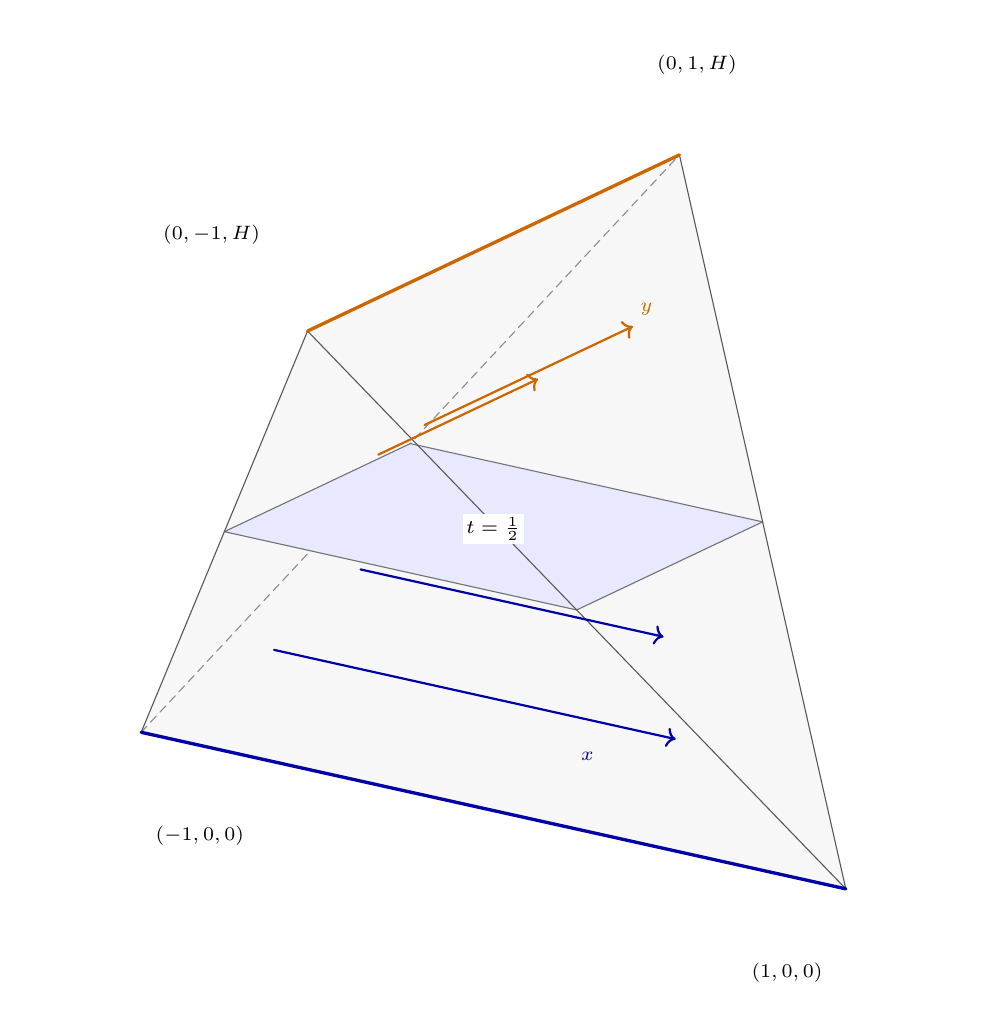
\begin{tikzpicture}[x=0.205\linewidth,y=0.205\linewidth,
      font=\scriptsize,line cap=round,line join=round]
      \coordinate (A) at (-1.8,0.4);   %
      \coordinate (B) at (1.8,-0.4);   %
      \coordinate (C) at (-0.95,2.45); %
      \coordinate (D) at (0.95,3.35);  %
      \coordinate (AC) at (-1.375,1.425);
      \coordinate (BC) at (0.425,1.025);
      \coordinate (BD) at (1.375,1.475);
      \coordinate (AD) at (-0.425,1.875);
      \fill[black!3] (A)--(B)--(D)--(C)--cycle;
      \draw[black!45,densely dashed] (A)--(D);
      \fill[blue!9] (AC)--(BC)--(BD)--(AD)--cycle;
      \draw[black!55,thin] (AC)--(BC)--(BD)--(AD)--cycle;
      \draw[black!65] (A)--(C)--(D)--(B)--cycle (B)--(C);
      \draw[blue!65!black,very thick] (A)--(B);
      \draw[orange!80!black,very thick] (C)--(D);
      \draw[->,blue!65!black,thick] (-1.121,0.821)--(0.931,0.365);
      \draw[->,blue!65!black,thick] (-0.679,1.232)--(0.869,0.888);
      \draw[->,orange!80!black,thick] (-0.352,1.970)--(0.712,2.474);
      \draw[->,orange!80!black,thick] (-0.5885,1.8185)--(0.2285,2.2055);
      \node[blue!65!black,anchor=north] at (0.48,0.35) {$x$};
      \node[orange!80!black,anchor=south west] at (0.70,2.48) {$y$};
      \node[fill=white,inner sep=1.3pt] at (0,1.44) {$t=\tfrac12$};
      \node at (-1.50,-0.13) {$(-1,0,0)$};
      \node at (1.50,-0.83) {$(1,0,0)$};
      \node at (-1.44,2.94) {$(0,-1,H)$};
      \node at (1.04,3.81) {$(0,1,H)$};
      \path[use as bounding box] (-2.38,-0.99) rectangle (2.38,4.00);
    \end{tikzpicture}\par
    {\scriptsize Physical coordinates $(x,y,Ht)$; $H=\sqrt{2}$.}
  \end{minipage}\hfill
  \begin{minipage}[t]{0.49\linewidth}
    \centering
    {\small\textbf{(b)} Matching after the tilt, $x=X$}\par\smallskip
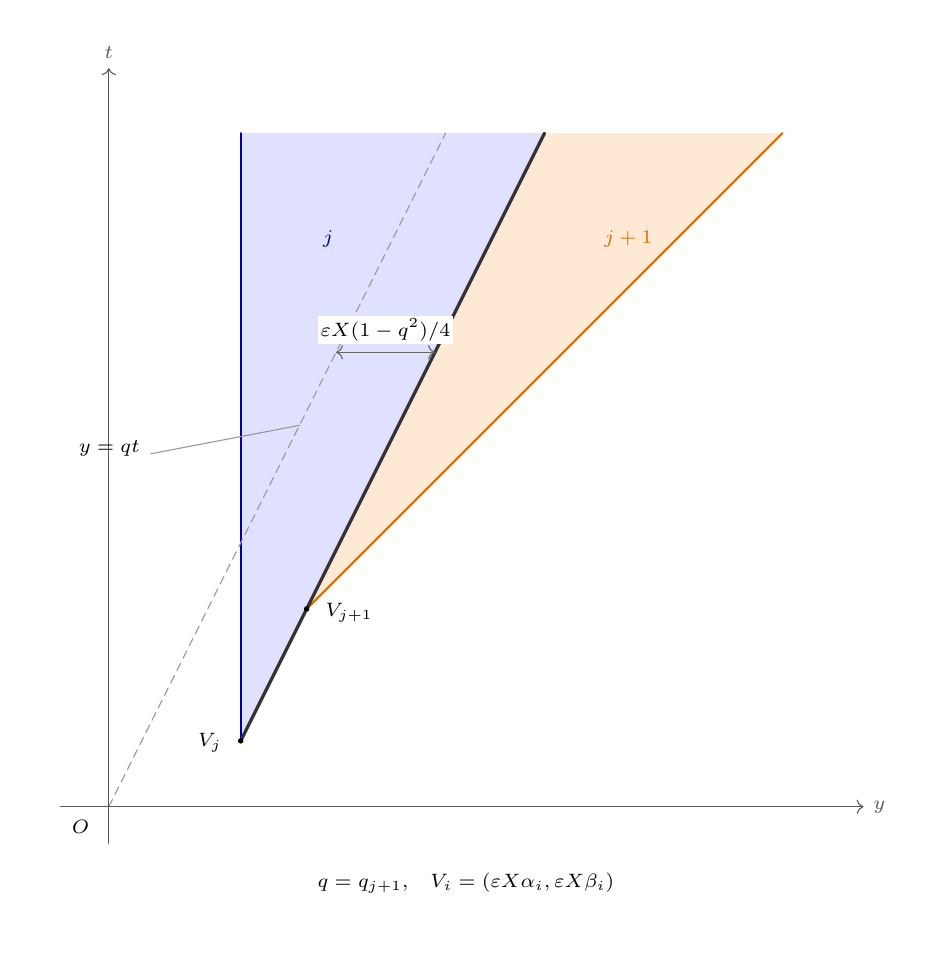
\begin{tikzpicture}[x=0.85\linewidth,y=0.85\linewidth,
  font=\scriptsize,line cap=round,line join=round]
  \coordinate (A) at (.1625,.08125);
  \coordinate (B) at (.24375,.24375);
  \coordinate (Ltop) at (.1625,.83);
  \coordinate (Mtop) at (.536875,.83);
  \coordinate (Rtop) at (.83,.83);
  \fill[blue!12] (A)--(Ltop)--(Mtop)--cycle;
  \fill[orange!17] (B)--(Mtop)--(Rtop)--cycle;
  \draw[blue!65!black,thick] (A)--(Ltop);
  \draw[orange!85!black,thick] (B)--(Rtop);
  \draw[black!80,very thick] (A)--(Mtop);
  \draw[black!40,densely dashed] (0,0)--(.415,.83);
  \draw[<->,black!60] (.28,.56)--(.401875,.56);
  \node[fill=white,inner sep=1pt,anchor=south] at (.3409375,.57)
    {$\eps X(1-q^2)/4$};
  \draw[->,black!65] (-.06,0)--(.93,0) node[right] {$y$};
  \draw[->,black!65] (0,-.045)--(0,.91) node[above] {$t$};
  \node[anchor=north east] at (-.012,-.005) {$O$};
  \fill (A) circle[radius=1pt];
  \fill (B) circle[radius=1pt];
  \node[anchor=east] at (.151,.079) {$V_j$};
  \node[anchor=west] at (.255,.239) {$V_{j+1}$};
  \node[blue!65!black] at (.27,.70) {$j$};
  \node[orange!85!black] at (.64,.70) {$j+1$};
  \node[anchor=south east,align=right] at (.05,.42) {$y=qt$};
  \draw[black!40,thin] (.052,.435)--(.235,.47);
  \node[anchor=north,align=center] at (.44,-.07)
    {$q=q_{j+1}$,\quad $V_i=(\eps X\alpha_i,\eps X\beta_i)$};
  \path[use as bounding box] (-.10,-.15) rectangle (1,.96);
\end{tikzpicture}\par
{\scriptsize The common supporting line is $y=qt+\eps X(1-q^2)/4$.}

  \end{minipage}
  \caption{(a) At zero tilt, cylinders parallel to the two opposite edges cover the lower and upper halves of $K$.
  (b) In the plane $x=X$, neighboring angular sectors have distinct translated vertices $V_j$ and $V_{j+1}$, but their sides at $q=q_{j+1}$ lie on the same line $y=qt+\eps X(1-q^2)/4$.
  The dashed line is $y=qt$, its zero-tilt position. Tilt and sector widths are exaggerated. Radial cutoffs are omitted; the colored regions end at the boundary of the displayed window.}
  \label{fig:construction}
\end{figure}


\section{Coverage of the entire tetrahedron}\label{sec:coverage}

The shared-boundary identity gives an angular sector in each family for
every point of $K$. The remaining task is to prove that at least one of the
two selected triangles has sufficient radial extent.

\begin{proposition}\label{prop:coverage}
For every $0<\eps\le\eta/2$, the $2n$ cylinders
\eqref{eq:first-family}--\eqref{eq:second-family}, with parameters
\eqref{eq:parameters}--\eqref{eq:cutoffs}, cover the closed tetrahedron $K$.
\end{proposition}
\begin{proof}
\emph{Choosing angular sectors.} Fix $(x,y,Ht)\in K$ and write $s=1-t$.
The intercept along $v_j$ is $(0,y_0,Ht_0)$, where
\begin{equation}\label{eq:lower-intercept}
 t_0=t-\eps x\beta_j,\qquad y_0=y-\eps x\alpha_j.
\end{equation}
Consider the finite sequence
\[
 F_i=q_it+\eps x\frac{1-q_i^2}{4}\qquad(0\le i\le n).
\]
Its endpoints are $F_0=-t\le y\le t=F_n$.
Choose the first index $i\ge1$ for which $F_i\ge y$, and set $j=i-1$.
Such an index exists because $F_n\ge y$. If $i=1$, then $F_j=F_0\le y$;
if $i>1$, minimality gives $F_j<y$. Thus
$F_j\le y\le F_{j+1}$, including when $y$ equals an extreme endpoint.
Using \eqref{eq:shared-boundaries}, these inequalities are exactly
\begin{equation}\label{eq:lower-sector}
 q_jt_0\le y_0\le q_{j+1}t_0.
\end{equation}
Subtracting their outer terms gives $0\le(q_{j+1}-q_j)t_0=\Delta t_0$.
Since $\Delta>0$, they force $t_0\ge0$.
Hence the selected first-family cylinder covers the point unless $t_0>T_j$.
This argument does not assume that the sequence $F_i$ is monotone.

For the second family, use the sequence
\[
 G_i=q_is-\eps y\frac{1-q_i^2}{4},\qquad G_0=-s\le x\le s=G_n.
\]
The same first-crossing choice gives an index $k$ for which
\begin{equation}\label{eq:upper-intercept}
 s_0=s+\eps y\beta_k\ge0,\qquad x_0=x+\eps y\alpha_k,\qquad
 q_ks_0\le x_0\le q_{k+1}s_0.
\end{equation}
This cylinder covers unless $s_0>T_k$.

\emph{Comparing the radial cutoffs.} It remains to show that the two selected radial cutoffs cannot both fail.
Suppose both selected cylinders miss the point.
Then $t_0,s_0>1/2$, and we can set
\[
 q=y_0/t_0\in[q_j,q_{j+1}],\qquad
 p=x_0/s_0\in[q_k,q_{k+1}].
\]
Since $|x|+|y|\le1$, \eqref{eq:coefficient-bounds} gives
\[
 t_0+s_0=1-\eps x\beta_j+\eps y\beta_k\le1+\eps/2.
\]
Thus each of $t_0,s_0$ lies between $1/2$ and $1/2+\eps/2$.
Using $y=t_0q+\eps x\alpha_j$ and $x=s_0p-\eps y\alpha_k$, we obtain
\begin{equation}\label{eq:rough-angles}
 |y-q/2|\le\eps,\qquad |x-p/2|\le\eps.
\end{equation}

Since $|\beta_j-q/2|\le\Delta/4$ and
$|\beta_k-p/2|\le\Delta/4$, \eqref{eq:rough-angles} gives
$|\beta_j-y|,|\beta_k-x|\le\eps+\Delta/4$.
Thus the intercept heights $t_0=t-\eps x\beta_j$ and
$s_0=s+\eps y\beta_k$ have opposite first-order changes
$-\eps xy$ and $+\eps xy$. This cancellation is the reason for choosing
$\beta_j$ close to $q/2$.

To control the remaining terms exactly, write $a=t_0-1/2$ and
$b=s_0-1/2$. The two radial excesses satisfy
\begin{align}
 a(1-\eps xq)+b(1+\eps yp)
 &=\eps^2(x^2\alpha_j+y^2\alpha_k)\notag\\
 &\quad-\eps x(\beta_j-q/2)+\eps y(\beta_k-p/2).
 \label{eq:radial-budget}
\end{align}
For completeness, $a+b=-\eps x\beta_j+\eps y\beta_k$, while the
intercept equations give
$q a=y-\eps x\alpha_j-q/2$ and
$p b=x+\eps y\alpha_k-p/2$. Substitute these three identities into the
left side of \eqref{eq:radial-budget}; the two mixed terms cancel.

For $0<\eps<1$, both factors multiplying $a$ and $b$ are at least
$1-\eps>0$. Since $a>\eps^2M_j$, $b>\eps^2M_k$ and $|x|+|y|\le1$, dividing
\eqref{eq:radial-budget} by $\eps^2$ yields
\begin{equation}\label{eq:failure-inequality}
 0>(M_j+M_k)(1-\eps)-\frac{\Delta}{4\eps}
                   -(x^2\alpha_j+y^2\alpha_k).
\end{equation}

We bound the last term without losing uniformity at the boundary.
From \eqref{eq:rough-angles} and $|x|,|y|\le1$, $|p|,|q|\le1$,
\[
 |x^2-p^2/4|,\ |y^2-q^2/4|\le\tfrac32\eps.
\]
For a point inside its interval,
\[
 \left|\alpha_j-\frac{1+q^2}{4}\right|\le\Delta/2,\qquad
 \left|\alpha_k-\frac{1+p^2}{4}\right|\le\Delta/2.
\]
Consequently
\begin{align*}
 x^2\alpha_j+y^2\alpha_k
 &\le\frac{p^2+q^2+2p^2q^2}{16}+\frac32\eps+\frac\Delta4\\
 &\le d(p)+d(q)+\frac32\eps+\frac\Delta4.
\end{align*}
The second inequality explains our choice of radial enlargement:
\[
 d(p)+d(q)-\frac{p^2+q^2+2p^2q^2}{16}
 =\frac{(p^2-q^2)^2}{16}\ge0.
\]
The cutoff definitions give
\[
 d(p)+d(q)+2\eta\le M_j+M_k\le\frac14+2\eta.
\]
Using $\Delta\le\eps^2$, the right side of \eqref{eq:failure-inequality} is therefore at least
\begin{equation}\label{eq:uniform-coverage-gap}
 2\eta-(2+2\eta)\eps-\frac{\eps^2}{4}.
\end{equation}
For $0<\eps\le\eta/2$ this is at least
$\eta-17\eta^2/16>0$, a contradiction.
All sector and cutoff inequalities are non-strict membership conditions. The argument applies to every point of the closed tetrahedron, including its faces, edges and vertices.
\end{proof}

We retain the numerical estimate with a variable margin for the later
construction in Section~\ref{sec:angular-cubic}.

\begin{corollary}[Quantitative coverage criterion]
\label{cor:quantitative-coverage}
Let $0<\tau<1$ and $\eta\ge0$. Choose an integer $n$ with
$\Delta=2/n\le\tau^2$, put $q_j=-1+j\Delta$, and define
$\alpha_j,\beta_j$ by \eqref{eq:axis-coefficients}. Use the triangles and
directions \eqref{eq:first-family}--\eqref{eq:second-family}, with
$\eps$ replaced by $\tau$ and with cutoffs
\[
 T_j=\frac12+\tau^2\left(\eta+\max_{q_j\le q\le q_{j+1}}d(q)\right).
\]
These $2n$ cylinders cover $K$ whenever
\begin{equation}\label{eq:variable-margin-budget}
 2\eta-(2+2\eta)\tau-\frac{\tau^2}{4}\ge0.
\end{equation}
\end{corollary}
\begin{proof}
The angular first-crossing argument is unchanged. If both selected caps
failed, their intercept heights would exceed $1/2$ and have sum at most
$1+\tau/2$. Thus the rough-angle estimates and the radial budget remain
valid with the same constants, independently of $\eta$. The only later
use of the margin is through
$d(p)+d(q)+2\eta\le M_j+M_k\le1/4+2\eta$.
Consequently the same calculation as
\eqref{eq:failure-inequality}--\eqref{eq:uniform-coverage-gap} gives
$0>2\eta-(2+2\eta)\tau-\tau^2/4$, contradicting
\eqref{eq:variable-margin-budget}.
\end{proof}

For the fixed parameters of the main construction, the coverage threshold
$\eps\le1/2000$ will also guarantee strict area saving. We now bound
the area remainder explicitly, so no further choice of a smaller tilt
is needed.

\section{The strict area decrease}\label{sec:area}

Coverage is now established. We compare the perpendicular areas of the
tilted triangles with the two-triangle cost $H/2$. All error estimates below
are uniform over the intervals of the partition.

Let $S(\eps)$ denote the sum of the areas of all $2n$ perpendicular bases.
Each intercept triangle in \eqref{eq:first-family} and \eqref{eq:second-family} has physical area $H\Delta T_j^2/2$.
Orthogonal projection between planes multiplies area by the absolute inner product of their unit normals.
For either family, the factor is
\[
 [1+\eps^2(\alpha_j^2+H^2\beta_j^2)]^{-1/2}.
\]
We therefore have the exact finite formula
\begin{equation}\label{eq:exact-area-sum}
 \frac{S(\eps)}H=
 \sum_{j=0}^{n-1}\Delta T_j^2
   [1+\eps^2(\alpha_j^2+2\beta_j^2)]^{-1/2}.
\end{equation}

\Needspace{5\baselineskip}
\begin{proposition}\label{prop:area-expansion}
For the construction \eqref{eq:parameters}--\eqref{eq:second-family} and
$0<\eps\le1$,
\[
 \left|\frac{S(\eps)}H-\frac12-
       \left(2\eta-\frac1{240}\right)\eps^2\right|
 \le 2\eps^4.
\]
\end{proposition}
\begin{proof}
Put $A_j=\alpha_j^2+2\beta_j^2$ and
\[
 f_j(z)=(\tfrac12+M_jz)^2(1+A_jz)^{-1/2}.
\]
The bounds \eqref{eq:coefficient-bounds} imply $0\le A_j\le1$ and
$0\le M_j\le1/4$. For $0\le z\le1$, direct differentiation gives
\begin{align*}
 f_j''(z)&=\frac{2M_j^2}{(1+A_jz)^{1/2}}
 -\frac{2A_jM_j(1/2+M_jz)}{(1+A_jz)^{3/2}}\\
 &\qquad+\frac{3A_j^2(1/2+M_jz)^2}{4(1+A_jz)^{5/2}},
\end{align*}
so
\[
 |f_j''(z)|\le\frac18+\frac38+\frac{27}{64}=\frac{59}{64}.
\]
Taylor's theorem at $z=0$, followed by \eqref{eq:exact-area-sum} and
$\sum_j\Delta=2$, now gives
\begin{equation}\label{eq:taylor-bound}
 \left|\frac{S(\eps)}H-\frac12-
 \eps^2\sum_j\Delta\left(M_j-\frac{A_j}{8}\right)\right|
 \le\frac{59}{64}\eps^4.
\end{equation}
In particular, the growing number of sectors causes no loss in the error
bound: each remainder is weighted by its interval length.

It remains to replace this finite sum by a polynomial integral. For
$q\in[q_j,q_{j+1}]$, set
\[
 A(q)=\frac{(1+q^2)^2}{16}+\frac{q^2}{2}.
\]
Since $|d'|\le3/8$ on $[-1,1]$,
\[
 |M_j-\eta-d(q)|\le\frac38\Delta.
\]
Also
$|\alpha_j-(1+q^2)/4|\le\Delta/2$ and
$|\beta_j-q/2|\le\Delta/4$.
The quantities in each of these differences have absolute value at most
$1/2$, so $|A_j-A(q)|\le\Delta$. Therefore
\[
 \left|M_j-\frac{A_j}{8}
     -\left(\eta+d(q)-\frac{A(q)}8\right)\right|
 \le\frac12\Delta.
\]
Integrating over all intervals shows that replacing the sum in
\eqref{eq:taylor-bound} by
$\int_{-1}^1(\eta+d(q)-A(q)/8)\,dq$ costs at most
$\eps^2\Delta\le\eps^4$. Finally,
\[
 \int_{-1}^1d(q)\,dq=\frac1{15},\qquad
 \int_{-1}^1A(q)\,dq=\frac{17}{30},
\]
so this integral equals $2\eta-1/240$. The combined error is at most
$(59/64+1)\eps^4<2\eps^4$, as claimed.
\end{proof}

\begin{proof}[Proof of \cref{thm:counterexample}]
The projection minimum is \cref{lem:projection-minimum}.
The construction in \cref{sec:construction} has exactly $2n$ compact
triangular perpendicular bases, and \cref{prop:coverage} proves that its
cylinders cover $K$ for $0<\eps\le\eta/2=1/2000$.
Since $\eta=1/1000$, \cref{prop:area-expansion} gives
\[
 \frac{S(\eps)}H
 \le\frac12-\frac{13}{6000}\eps^2+2\eps^4<\frac12
 \qquad(0<\eps\le1/2000),
\]
where the strict inequality follows from
$2\eps^2\le1/2{,}000{,}000<13/6000$.
The same proposition gives the expansion and its stated remainder.
\end{proof}

The same computation also controls a margin chosen separately for each
tilt. This will let us make the margin vanish without hiding its area cost.

\begin{corollary}[Area estimate with a variable margin]
\label{cor:variable-margin-area}
Let $0<\tau\le1$ and $0\le\eta\le1/8$. Choose an integer $n$ with
$\Delta=2/n\le\tau^2$, put $q_j=-1+j\Delta$, and use the secant
coefficients \eqref{eq:axis-coefficients} and cutoffs
\[
 T_j=\frac12+\tau^2\left(\eta+\max_{q_j\le q\le q_{j+1}}d(q)\right).
\]
For the two families \eqref{eq:first-family}--\eqref{eq:second-family},
with $\eps$ replaced by $\tau$, their total perpendicular base area $C$
satisfies
\begin{equation}\label{eq:variable-margin-area}
 \left|\frac CH-\frac12-
       \left(2\eta-\frac1{240}\right)\tau^2\right|
 \le\frac{59}{64}\tau^4+\tau^2\Delta
 \le2\tau^4.
\end{equation}
The estimate is uniform over all these choices; it does not assume
that the cylinders cover $K$.
\end{corollary}
\begin{proof}
Here $M_j=\eta+\max_{[q_j,q_{j+1}]}d\le1/4$ and $A_j\le1$,
so the preceding second-derivative bound applies unchanged. It gives
the Taylor error $59\tau^4/64$. In the comparison with
$\eta+d(q)-A(q)/8$, the constant $\eta$ cancels, leaving an error
at most $\Delta/2$ at each angular point. Integration therefore costs
at most $\tau^2\Delta$. Neither bound requires $\eta$ to be fixed
as $\tau$ varies.
\end{proof}

\section{Other caps and angular partitions}
\label{ext:cap-section}

The triangular construction leaves two choices available: how to end a
sector radially, and where to sample its direction.  The same balance
between radial enlargement and perpendicular projection permits curved
caps, smaller fixed margins, and sectors centred at the sampling nodes.
We continue to use
\[
 H=\sqrt2,\qquad
 K=\{(x,y,Hs):0\le s\le1,\ |x|\le1-s,\ |y|\le s\},
 \qquad d(q)=\frac{q^2+q^4}{16}.
\]
Thus $A_{\min}(K)=H$.  All the cylinders below are specified by an
intercept set and a nonzero direction; their bases are the perpendicular
projections of the intercept sets.

\subsection{A fixed positive margin}

The following criterion isolates what the angular construction uses.
Continuity of the displaced boundaries chooses a sector, and a positive
quadratic margin ensures that the two chosen radial caps cannot both fail.
The partition may be nonuniform, and its number of intervals need not
satisfy an upper bound.

\begin{theorem}[Compatible boundaries and radial caps]
\label{ext:general-cap}
Let $\tau>0$ tend to zero through any set accumulating at zero.
For each $\tau$, choose a finite partition
$-1=q_0<\cdots<q_m=1$, constants $\alpha_j,\beta_j$, and positive
continuous functions $R_j$ on $I_j=[q_{j-1},q_j]$.
Suppose that $L(q)=\alpha_j-q\beta_j$ is continuous on $[-1,1]$
and $L(-1)=L(1)=0$.  Suppose also, uniformly for every $j$ and
$q\in I_j$, that
\begin{align}
 \beta_j&=q/2+O(\tau^2),&
 \alpha_j&=(1+q^2)/4+O(\tau^2),\label{ext:coefficient-hypotheses}\\
 R_j(q)&=\tfrac12+\tau^2\bigl(d(q)+\eta\bigr)+O(\tau^4),
 &&0<\eta<1/480.\label{ext:cap-hypothesis}
\end{align}
Here $\eta$ is fixed, and all error constants and their common range of
validity are independent of $\tau,j,q$.
Define
\begin{align*}
 P_j^-&=\{(0,qS,HS):q\in I_j,\ 0\le S\le R_j(q)\},&
 v_j^-&=(1,\tau\alpha_j,H\tau\beta_j),\\
 P_j^+&=\{(qT,0,H(1-T)):q\in I_j,\ 0\le T\le R_j(q)\},&
 v_j^+&=(-\tau\alpha_j,1,H\tau\beta_j).
\end{align*}
For every sufficiently small admissible $\tau$, the $2m$ cylinders
$P_j^-+\mathbb Rv_j^-$ and $P_j^++\mathbb Rv_j^+$ cover the closed
tetrahedron $K$.  Their bases are compact, and their total area $C_\tau$
satisfies
\begin{equation}\label{ext:general-cost}
 \frac{C_\tau}{H}
 =\frac12+\left(2\eta-\frac1{240}\right)\tau^2+O(\tau^4).
\end{equation}
If each $R_j$ is constant, every base is a triangle.
The threshold and error constant may depend on $\eta$ and the uniform
constants in the hypotheses, but not on $m$.
\end{theorem}

\begin{proof}
Fix $(x,y,Hs)\in K$.  The continuous piecewise affine function
$q\mapsto qs+\tau xL(q)$ has outer values $-s,s$, which bracket $y$.
Choose the first partition node after $q_0$ whose value is at least $y$.
Its preceding value is at most $y$, by the initial endpoint inequality
or by minimality.  On the selected interval $I_j$, put
\[
 S=s-\tau x\beta_j,\qquad Y=y-\tau x\alpha_j.
\]
The crossing inequalities say $q_{j-1}S\le Y\le q_jS$, so $S\ge0$.
If $S=0$, then $Y=0$ and the selected cylinder already covers the point.
Otherwise $Y=qS$ for some $q\in I_j$.
Applying the same argument to
$p\mapsto p(1-s)-\tau yL(p)$ gives an interval $I_i$ and
\[
 T=1-s+\tau y\beta_i\ge0,\qquad
 X=x+\tau y\alpha_i=pT,\qquad p\in I_i.
\]
Again $T=0$ already gives coverage.  It remains to exclude
$S>R_j(q)$ and $T>R_i(p)$ simultaneously.

Assume these failures.  For sufficiently small $\tau$, the fixed
positive margin and the uniform cap error imply $S,T>1/2$.
Since $S+T=1+\tau(y\beta_i-x\beta_j)=1+O(\tau)$, each equals
$1/2+O(\tau)$.  The intercept equations then give
$y=q/2+O(\tau)$ and $x=p/2+O(\tau)$.
Write $e_j=\beta_j-q/2$ and $e_i=\beta_i-p/2$.
The same complementary radial balance as in the triangular construction
now has explicit sampling errors:
\begin{align*}
 s-\tau xy
 &=\tfrac12+(S-\tfrac12)(1-\tau xq)
       -\tau^2x^2\alpha_j+\tau xe_j,\\
 1-s+\tau xy
 &=\tfrac12+(T-\tfrac12)(1+\tau yp)
       -\tau^2y^2\alpha_i-\tau ye_i.
\end{align*}
These identities follow by substituting
$y=qS+\tau x\alpha_j$ and $x=pT-\tau y\alpha_i$.
Their left sides sum to one, and both factors multiplying the radial
excesses are positive for small $\tau$.  Substitute the strict cap
failures, divide by $\tau^2$, and use $e_i,e_j=O(\tau^2)$ to obtain
\[
 0> d(q)+d(p)+2\eta-x^2\alpha_j-y^2\alpha_i+O(\tau)
   =2\eta+\frac{(p^2-q^2)^2}{16}+O(\tau).
\]
The error is uniform.  This is impossible for sufficiently small
$\tau$, proving coverage, including the boundary.

The parametrizations of $P_j^-$ and $P_j^+$ have area Jacobians $HS$
and $HT$, respectively, and are one-to-one off their tips.
Projection multiplies area in either intercept plane by
$[1+\tau^2(\alpha_j^2+2\beta_j^2)]^{-1/2}$.
Consequently
\[
 \frac{C_\tau}{H}=
 \sum_j\int_{I_j}\frac{R_j(q)^2}
 {\sqrt{1+\tau^2(\alpha_j^2+2\beta_j^2)}}\,dq.
\]
Uniform expansion of the integrand gives
\[
 \frac14+\tau^2\left[
 d(q)+\eta-\frac18\left(\frac{(1+q^2)^2}{16}+\frac{q^2}{2}\right)
 \right]+O(\tau^4).
\]
The total angular length is two, so integration preserves the uniform
fourth-order remainder regardless of the number of intervals.  Finally
\[
 \int_{-1}^1d(q)\,dq=\frac1{15},\qquad
 \frac18\int_{-1}^1\left(\frac{(1+q^2)^2}{16}+\frac{q^2}{2}\right)dq
 =\frac{17}{240},
\]
which proves \eqref{ext:general-cost}.  Each parameter domain is compact;
its continuous image and perpendicular projection are compact as well.
Projection is invertible between the intercept plane and the base plane,
so a constant cap gives a nondegenerate triangle.
\end{proof}

\subsection{Triangular and curved apertures}
\label{ext:apertures}

For an ordinary interval $I=[l,r]$, use
\begin{equation}\label{ext:ordinary-secants}
 \alpha_I=\frac{1+lr}{4},\qquad \beta_I=\frac{l+r}{4}.
\end{equation}
The identity $\alpha_I-q\beta_I=(1-q^2)/4$ at both endpoints
matches adjacent boundaries exactly.  If the maximum interval length
is at most $M\tau^2$, for fixed $M$, then
\eqref{ext:coefficient-hypotheses} holds uniformly.
With $r_I=(l+r)/2$, each of the following choices satisfies
\eqref{ext:cap-hypothesis}:
\begin{align}
 R_I(q)&=\tfrac12+\tau^2\bigl(d(r_I)+\eta\bigr),
 &&\text{midpoint triangles},\label{ext:midpoint-cap}\\
 R_I(q)&=\tfrac12+\tau^2\bigl(\max_{u\in I}d(u)+\eta\bigr),
 &&\text{maximum triangles},\label{ext:maximum-cap}\\
 R_I(q)&=\tfrac12+\tau^2\bigl(d(q)+\eta\bigr),
 &&\text{continuous radial caps},\label{ext:radial-cap}\\
 R_I(q)&=\sqrt{\tfrac14+\tau^2\bigl(d(q)+\eta\bigr)},
 &&\text{squared-radius caps}.\label{ext:squared-cap}
\end{align}
Indeed, $d$ has bounded derivative on $[-1,1]$, so replacing $d(q)$
by its midpoint value or its cell maximum costs $O(\tau^2)$ inside
the parentheses.  For \eqref{ext:squared-cap}, Taylor expansion at
$1/4$ gives the required fourth-order error.  Thus all four choices
have the area formula \eqref{ext:general-cost}.  The first two give
triangles; the last two give compact radial sectors.

Another choice specifies the radial enlargement through the transverse
intercept.  Put $D(Y)=Y^2/4+Y^4$.  For $b=3/4$ or $b=1$, retain the
bounded aperture
\begin{equation}\label{ext:cartesian-aperture}
 0\le S\le b,\qquad S\le\tfrac12+\tau^2\bigl(D(qS)+\eta\bigr).
\end{equation}
For small $\tau$, this is exactly $0\le S\le R(q)$, where $R$ is
continuous and satisfies \eqref{ext:cap-hypothesis}.  To verify this,
consider $f(S)=S-1/2-\tau^2(D(qS)+\eta)$ on $[0,1]$.  Uniformly in
$|q|\le1$,
\[
 f'(S)=1-\tau^2(q^2S/2+4q^4S^3)\ge1-\tfrac92\tau^2.
\]
For small $\tau$, $f$ is strictly increasing, is negative at $1/2$,
and is positive at $3/4$.  Its unique zero $R(q)$ lies between these
values and depends continuously on $q$.  Its defining equation first
gives $R(q)-1/2=O(\tau^2)$, and then
\[
 D(qR(q))=D(q/2)+O(\tau^2)=d(q)+O(\tau^2),
\]
which proves the cap expansion.  The outer bound in
\eqref{ext:cartesian-aperture} is part of the definition: without it,
the quartic inequality can admit a second, unbounded component.

The common conclusion is easiest to compare in the fixed tetrahedron $K$:
for each fixed $0<\eta<1/480$, every cap above has normalized total area
\eqref{ext:general-cost}.  Its threshold is uniform over partitions whose
maximum interval length is at most $M\tau^2$, for a fixed $M$.
For example, an equal partition with any integer $m\ge2/\tau^2$ gives
exactly $2m$ cylinders, with the same threshold and error constant as the
mesh is refined.  Each cover is finite; no further limit in the number
of cylinders is needed after choosing the tilt and mesh.

The squared-radius and Cartesian formulas also explain the geometry in
two different ways.  Appendix~\ref{ext:squared-direct} compares the two
radial squares, while Appendix~\ref{ext:cartesian-direct} uses a
discriminant to estimate the intercept height without locating the
perturbed interface.  These are alternative proofs of cases already
covered by Theorem~\ref{ext:general-cap}.  Exact counts and costs for
several rescaled parameter choices are collected in
Appendix~\ref{ext:scaling-specializations}.

\subsection{Sampling at the endpoints}
\label{ext:endpoint-sectors}

The compatibility condition also permits directions sampled at nodes
rather than along secants of each sector.  Let $k>1$ be an integer,
$\tau=1/k$, $n=k^2$, and $q_j=-1+2j/n$ for $0\le j\le n$.
Put $\lambda_0=-1$, $\lambda_{n+1}=1$, and
$\lambda_j=(q_{j-1}+q_j)/2$ for $1\le j\le n$.
Use the sectors $[\lambda_j,\lambda_{j+1}]$ and parameters
\[
 \beta_j=q_j/2,\qquad \alpha_j=(1+q_j^2)/4,\qquad
 R_j=\tfrac12+\tau^2\bigl(d(q_j)+1/1000\bigr).
\]
At an interior boundary,
$\alpha_j-\alpha_{j-1}=\lambda_j(\beta_j-\beta_{j-1})$;
at the exterior boundaries $\alpha_j-\lambda\beta_j=0$.
Thus the piecewise affine boundary function is continuous and vanishes
at both ends.  Every angular point of the $j$th sector is within $\tau^2$
of $q_j$, so all the hypotheses of Theorem~\ref{ext:general-cap} hold.
There are $n+1$ sectors, with widths $\tau^2$ at the two ends and
$2\tau^2$ in the interior.  Consequently, for all sufficiently large $k$,
this construction covers $K$ with exactly $2(k^2+1)$ triangular bases
and normalized total area
\begin{equation}\label{ext:endpoint-cost}
 \frac{C_\tau}{A_{\min}(K)}
 =\frac12-\frac{13}{6000}\tau^2+O(\tau^4).
\end{equation}
The half-width end sectors preserve the exact exterior boundaries.
Appendix~\ref{ext:endpoint-direct} gives a complementary radial identity
that verifies their coverage directly, and
Appendix~\ref{ext:endpoint-scaled} records the corresponding absolute
area at edge length $\sqrt2$.

\section{A vanishing radial margin}
\label{sec:angular-cubic}

For a fixed positive margin, the normalized area coefficient is
$2\eta-1/240$. We now let the margin tend to zero with the tilt and
obtain the coefficient $-1/240$ in a single family of finite triangular
covers. The extra radial enlargement is cubic in the tilt. Its positive
cubic area term explains why coverage persists on a much wider interval
than the interval on which we prove a saving.

The fixed-margin theorem, Theorem~\ref{ext:general-cap}, cannot be
applied uniformly when $\eta$ tends to zero. Instead we use the explicit
coverage budget in Corollary~\ref{cor:quantitative-coverage} and the
uniform area estimate in Corollary~\ref{cor:variable-margin-area}.
We keep the edge-two tetrahedron $K$ and the same slope coordinates.

\begin{proposition}\label{prop:angular-cubic}
For every $0<\tau\le1$, the tetrahedron $K$ admits a cover by
$2\lceil8/\tau^2\rceil$ cylinders with compact, nondegenerate triangular
perpendicular bases. Their total base area $C_\tau$ satisfies
\begin{equation}\label{eq:angular-cubic-cost}
 \left|\frac{C_\tau}{H}-\frac12+\frac{\tau^2}{240}
                   -\frac{25}{2}\tau^3\right|
 \le2\tau^4\qquad(0<\tau\le1/50).
\end{equation}
In particular, $C_\tau<A_{\min}(K)/2$ for $0<\tau\le1/4000$, and
\[
 \frac{C_\tau}{A_{\min}(K)}
 =\frac12-\frac{\tau^2}{240}+O(\tau^3)
 \qquad(\tau\downarrow0).
\]
\end{proposition}
\begin{proof}
Put
\[
 N=\left\lceil\frac8{\tau^2}\right\rceil,\qquad
 \Delta=\frac2N\le\frac{\tau^2}{4},\qquad
 q_j=-1+j\Delta\quad(0\le j\le N).
\]
Use the secant coefficients \eqref{eq:axis-coefficients}, and set
\begin{equation}\label{eq:cubic-caps}
 d_j=\max_{q_j\le q\le q_{j+1}}d(q),\qquad
 T_j=\frac12+\tau^2d_j+\frac{25}{4}\tau^3
 \qquad(0\le j<N).
\end{equation}
The intercept triangles and directions are
\eqref{eq:first-family}--\eqref{eq:second-family}, with $\eps$ replaced
by $\tau$ and these cutoffs. They give exactly $2N$ cylinders.
Their intercept triangles have positive area, and the normal component
of each axis is one, so their perpendicular bases are compact
nondegenerate triangles as before.

\emph{Coverage.} For $0<\tau\le1/2$, take $\eta=25\tau/4$ in
Corollary~\ref{cor:quantitative-coverage}. Its sufficient budget is
\[
 2\eta-(2+2\eta)\tau-\frac{\tau^2}{4}
 =\tau\left(\frac{21}{2}-\frac{51}{4}\tau\right)
 \ge\frac{33}{8}\tau>0.
\]
Thus the cylinders cover $K$ throughout this range.

For $1/2\le\tau\le1$, the enlarged triangles are already large enough
for the first family alone. Indeed, for $(x,y,Ht)\in K$ the first-crossing
argument selects a first-family sector with intercept height
\[
 0\le t_0=t-\tau x\beta_j
 \le t+\frac{\tau}{2}|x|
 \le t+\frac{\tau}{2}(1-t)\le1.
\]
Its cutoff obeys
$T_j\ge1/2+(25/4)\tau^3\ge41/32>1$.
The selected cylinder therefore contains the point. Both arguments use
non-strict angular membership conditions, so they cover the closed
body, including its boundary.

\emph{Area.} For $0<\tau\le1/50$, the margin $\eta=25\tau/4$ lies
in $[0,1/8]$. Corollary~\ref{cor:variable-margin-area} consequently gives
\[
 \left|\frac{C_\tau}{H}-\frac12-
       \left(\frac{25}{2}\tau-\frac1{240}\right)\tau^2\right|
 \le2\tau^4,
\]
which is \eqref{eq:angular-cubic-cost}. This application is uniform
although the margin varies with the tilt. If $0<\tau\le1/4000$, then
\[
 \frac{25}{2}\tau+2\tau^2
 \le\frac1{320}+\frac1{8{,}000{,}000}<\frac1{240}.
\]
The negative quadratic term therefore exceeds both the positive cubic
term and the error, giving $C_\tau<H/2=A_{\min}(K)/2$.
\end{proof}

The equivalent edge-four construction, with its full coverage interval,
exact cylinder count and scaled area estimates, is recorded in
Remark~\ref{rem:angular-cubic-scale} of Appendix~\ref{ext:scaling-specializations}.

\appendix
\section{Alternative coverage and area calculations}
\label{ext:alternate-estimates}

The fixed-margin criterion already proves coverage for the cap choices
in Section~\ref{ext:cap-section}.  The following direct calculations
explain three particular features: why squared-radius caps suit a
comparison of radial squares, how a Cartesian discriminant avoids
locating the perturbed interface, and how node-centred sectors retain
the complementary radial cancellation.  They are independent
explanations of those cases, rather than inputs to the main construction
or the vanishing-margin argument.

\subsection{Squared radii}
\label{ext:squared-direct}
Let $n$ be a positive integer, put $k=1/n$, use $n^2$ equal intervals,
and write their width as
$\Delta=2k^2$.  Put
\[
 M_I=(l+r)/2=2\beta_I,\qquad B_I=(1+lr)/2=2\alpha_I,
 \qquad f(q)=(q^2+q^4)/4.
\]
The squared-radius cap \eqref{ext:squared-cap}, with
$\tau=2k$ and $\eta=1/960$, is
$R(q)^2=1/4+k^2(f(q)+1/240)$.
The elementary secant identity is exact:
\begin{equation}\label{ext:squared-identity}
 2B_I-M_I^2=1-\frac{\Delta^2}{4}.
\end{equation}
For the two angularly selected intercepts, write
\[
 S=s-kxM_I,\qquad y=qS+kxB_I,
 \qquad T=1-s+kyM_J,\qquad x=pT-kyB_J.
\]
The crossing argument supplies $S,T\ge0$.  If both radial caps fail,
then $S,T>1/2$ and $u=s-1/2=O(k)$.
Since $M_I=q+O(k^2)$ and $M_J=p+O(k^2)$, substitution in
\[
 S^2=s^2-2kxSM_I-k^2x^2M_I^2,
 \qquad
 T^2=(1-s)^2+2kyTM_J-k^2y^2M_J^2
\]
and use of \eqref{ext:squared-identity} give the uniform expansions
\begin{align}
 S^2&=\tfrac14+u+u^2-2kxy+k^2x^2+O(k^3),\nonumber\\
 T^2&=\tfrac14-u+u^2+2kxy+k^2y^2+O(k^3).
 \label{ext:squared-expansions}
\end{align}
For example $SM_I=y-kxB_I+O(k^2)$, and the second identity uses
$TM_J=x+kyB_J+O(k^2)$.
Since $|M_I|,|M_J|\le1$, the failures $S,T>1/2$ first give
$|u|\le k$.  The first strict lower bound on $S^2$ then gives
$u-2kxy\ge-Ck^2$, and the second gives
$u-2kxy\le Ck^2$, for a uniform constant $C$.
Thus $u=2kxy+O(k^2)$.  Adding \eqref{ext:squared-expansions} now yields
\[
 \frac{S^2+T^2-1/2}{k^2}
 =x^2+y^2+8x^2y^2+O(k).
\]
On the other hand $q=2y+O(k)$ and $p=2x+O(k)$, so
\[
 f(q)+f(p)=x^2+y^2+4(x^4+y^4)+O(k)
 \ge x^2+y^2+8x^2y^2+O(k).
\]
The failed caps require the previous quotient to exceed
$f(q)+f(p)+2/240$, a contradiction for small $k$.

Let $C_k$ denote the sum of the perpendicular base areas of all $2n^2$
cylinders. The two families have equal total area, and the square in the
cap makes the radial integration exact before the projection factor is
expanded:
\[
 \frac{C_k}{2H}=
 \sum_I\int_I
 \frac{\frac12[\frac14+k^2(f(q)+1/240)]}
 {\sqrt{1+k^2(B_I^2+2M_I^2)}}\,dq
 =\frac14+k^2\left(\frac1{240}-\frac1{120}\right)+O(k^4).
\]
The squared cap therefore supplies both the coverage comparison and
the exact radial part of the area integral.

\subsection{A Cartesian discriminant}
\label{ext:cartesian-direct}
For an equal sector $I=[l,r]$ of width $\Delta$, the coefficients
\eqref{ext:ordinary-secants} satisfy
\[
 \beta_I^2-\alpha_I+1/4=\Delta^2/16.
\]
Suppose the angular crossing for one family has given
\[
 S=T-\delta\beta_I\ge0,\qquad
 Y_0=Y-\delta\alpha_I,\qquad lS\le Y_0\le rS.
\]
Here $(T,Y,\delta)=(s,y,\tau x)$ in the first family and
$(1-s,x,-\tau y)$ in the second.  Because $2\beta_I$ is the sector
midpoint, $|2\beta_IS-Y_0|\le\Delta S/2$.  Consequently
\begin{align}
 Q&:=T^2-\delta Y+\delta^2/4\nonumber\\
  &=S^2+\delta(2\beta_IS-Y_0)+\delta^2\Delta^2/16
    \ge (S-|\delta|\Delta/4)^2.
 \label{ext:cartesian-discriminant}
\end{align}
In particular $\sqrt Q\ge S-|\delta|\Delta/4$.
Take the Cartesian cap \eqref{ext:cartesian-aperture} with $b=1$,
fixed $\eta>0$, and $\Delta=O(\tau^2)$.
Since $0\le\alpha_I\le1/2$, $|Y|\le1$ and $|\delta|\le\tau$,
we have $|Y_0|\le1+\tau/2$.  For $\tau\le1$, this gives
$D(Y_0)\le D(3/2)=45/8$.  Hence the polynomial upper bound is less
than one whenever $\tau^2(45/8+\eta)<1/2$.
Failure of the selected cylinder therefore
implies $S>1/2+\tau^2(D(Y_0)+\eta)$ even if the outer bound $S\le1$
failed.  Since $Y_0=Y+O(\tau)$ and $|\delta|\Delta=O(\tau^3)$,
\eqref{ext:cartesian-discriminant} gives
\[
 \sqrt Q>\tfrac12+\tau^2\bigl(D(Y)+\eta/2\bigr)
\]
for sufficiently small $\tau$, uniformly in both families.
If both failed, squaring these positive lower bounds and discarding
their nonnegative fourth-order terms would give
\begin{align*}
 s^2&>\tfrac14+\tau xy+
          \tau^2\bigl(D(y)+\eta/2-x^2/4\bigr),\\
 (1-s)^2&>\tfrac14-\tau xy+
          \tau^2\bigl(D(x)+\eta/2-y^2/4\bigr).
\end{align*}
The right sides are positive for small $\tau$.  Expanding their square
roots with $\sqrt{1/4+v}=1/2+v-v^2+O(v^3)$ shows that their sum is
\[
 1+\tau^2\bigl(D(x)+D(y)+\eta-(x^2+y^2)/4-2x^2y^2\bigr)
       +O(\tau^3)
 =1+\tau^2\bigl((x^2-y^2)^2+\eta\bigr)+O(\tau^3)>1,
\]
contradicting $s+(1-s)=1$.

For either outer bound $b\in\{3/4,1\}$, the Cartesian aperture admits a
direct area calculation without changing to angular variables at the
boundary.  In the intercept coordinates $(Y,S)$, put
\[
 \mathcal D_\tau=\{0\le S\le b,\ |Y|\le S,
            \ S\le1/2+\tau^2(D(Y)+\eta)\},\qquad
 \mathcal D_0=\{0\le S\le1/2,\ |Y|\le S\}.
\]
For $|Y|\le1/2$ the added vertical length is exactly
$\tau^2(D(Y)+\eta)$ for small $\tau$.  Each remaining side region has
both width and height $O(\tau^2)$, because
$1/2<|Y|\le S\le1/2+O(\tau^2)$ there.  Thus
\[
 |\mathcal D_\tau|=\frac14+
 \tau^2\int_{-1/2}^{1/2}(D(Y)+\eta)\,dY+O(\tau^4).
\]
Expanding the projection factor over $\mathcal D_0$, and using
$Y=qS$ in its quadratic coefficient, gives the one-family cost
\[
 \frac14+\tau^2\left[
 \underbrace{\int_{-1/2}^{1/2}D(Y)\,dY}_{1/30}+\eta
 -\underbrace{\frac12\int_0^{1/2}S\,dS
   \int_{-1}^1\left(\frac{(1+q^2)^2}{16}+\frac{q^2}{2}\right)dq}_{17/480}
 \right]+O(\tau^4).
\]
Here the cost is divided by $H$ in the edge-two normalization.
The replacement of $\mathcal D_\tau$ by $\mathcal D_0$ changes the
quadratic coefficient by $O(\tau^2)$, and the coefficient sampling
error is also $O(\tau^2)$; both contribute only $O(\tau^4)$ to the
area.  Thus the normalized two-family cost is
$1/2+(2\eta-1/240)\tau^2+O(\tau^4)$, as in
\eqref{ext:general-cost}.  The Cartesian entries in
Appendix~\ref{ext:scaling-specializations} follow by substitution; the
edge-one discriminant and aperture are translated there as well.

\subsection{A direct check for node-centred sectors}
\label{ext:endpoint-direct}

Use the node-centred sectors of Section~\ref{ext:endpoint-sectors},
and write their tilt as $t=1/k$.  The radial cutoff at a sample node $q$
is $1/2+t^2(d(q)+1/1000)$, and each angular point of its sector lies
within $t^2$ of $q$.  If the two selected sample nodes are $q,p$, write
\[
 S=s-txq/2,\quad y=qS+tx\alpha(q)+e,
 \qquad
 T=1-s+typ/2,\quad x=pT-ty\alpha(p)+e_*,
\]
where $|e|\le St^2$, $|e_*|\le Tt^2$, and
$\alpha(q)=(1+q^2)/4$.  Direct substitution gives
\begin{align*}
 s-txy&=\tfrac12+(S-\tfrac12)(1-tqx)-t^2\alpha(q)x^2-txe,\\
 1-s+txy&=\tfrac12+(T-\tfrac12)(1+tpy)-t^2\alpha(p)y^2+tye_*.
\end{align*}
If both radial caps failed along a sequence $t\to0$, then $S,T>1/2$ and
$S+T=1+t(yp-xq)/2=1+O(t)$, so $S,T\to1/2$.
Passing to a subsequence with $q\to q_0$, $p\to p_0$ gives
$y\to q_0/2$, $x\to p_0/2$, while $e/t,e_*/t\to0$.
Adding the identities and dividing by $t^2$ would therefore imply
\[
 0\ge\frac2{1000}+\frac{(q_0^2-p_0^2)^2}{16}>0.
\]
This complementary identity gives a second explanation for why the
half-width endpoint sectors still cover the boundary.

\section{Counts and formulas under changes of scale}
\label{ext:scaling-specializations}

The constructions in the main text use the edge-two tetrahedron $K$.
A similarity of ratio $a/2$ produces a regular tetrahedron of edge length
$a$: it multiplies every base area and the minimum projection area by
$(a/2)^2$, while preserving the number of cylinders and the normalized
cost.  This appendix records several parameter choices and their
coordinate dictionaries.

\subsection{Secant sectors}
\label{ext:secant-specializations}

In the following table, every row uses an equal partition with $m$ intervals
and hence exactly $2m$ cylinders.  The body has edge length $a$ and is
obtained from $K$ by a similarity of ratio $a/2$; accordingly the area
is reported as $C/A_{\min}$.  Each statement holds for all sufficiently
large indicated integers or all sufficiently small indicated positive
real parameters.  Every displayed remainder is fourth order in the
displayed tilt parameter, uniformly over the permitted finer meshes.
\begin{center}
\small
\renewcommand{\arraystretch}{1.3}
\begin{tabular}{lllll}
\toprule
Cap & $a$ & $(\tau,\eta)$ & $m$ & $C/A_{\min}$\\
\midrule
Midpoint & $4$ & $(2/n,1/1920)$ & $2n^2$
 & $\frac12-\frac1{80n^2}+O(n^{-4})$\\
Midpoint & $1$ & $(\alpha,1/1000)$ & $\lceil\alpha^{-2}\rceil$
 & $\frac12-\frac{13}{6000}\alpha^2+O(\alpha^4)$\\
Midpoint & $2$ & $(1/n,1/1000)$ & $n^2$
 & $\frac12-\frac{13}{6000n^2}+O(n^{-4})$\\
Continuous & $2$ & $(c,1/1000)$ & any $m\ge2/c^2$
 & $\frac12-\frac{13}{6000}c^2+O(c^4)$\\
Squared radius & $2$ & $(2/n,1/960)$ & $n^2$
 & $\frac12-\frac1{120n^2}+O(n^{-4})$\\
Maximum & $1$ & $(1/(4n),1/960)$ & $n^2$
 & $\frac12-\frac1{7680n^2}+O(n^{-4})$\\
Cartesian, $b=3/4$ & $\sqrt2$ & $(\lambda/2,1/960)$
 & $\lceil\sqrt2/\lambda^2\rceil$
 & $\frac12-\frac{\lambda^2}{1920}+O(\lambda^4)$\\
Cartesian, $b=1$ & $1$ & $(1/(2n),1/1000)$ & $n^2$
 & $\frac12-\frac{13}{24000n^2}+O(n^{-4})$\\
\bottomrule
\end{tabular}
\end{center}
The table follows by substitution in \eqref{ext:general-cost}; in each
row the mesh is bounded by a fixed multiple of $\tau^2$.
For the continuous cap, $m=\lceil2/c^2\rceil$ gives the ceiling count,
whereas $c=1/n$ permits every integer $m\ge2n^2$, with the same
threshold and error constant.  The real-parameter midpoint row includes
the reciprocal-integer construction after dilation by two.
For the squared-radius row, the two families have equal area and each
costs $H[1/4+(1/240-1/120)n^{-2}+O(n^{-4})]$.
For the first Cartesian row, either family costs
$c_0/4-c_0\lambda^2/3840+O(\lambda^4)$ with $c_0=1/\sqrt2$.
These are genuine finite covers: the positive margin is fixed first,
then a sufficiently small tilt and the specified finite mesh are chosen.
No further limit in the number of cylinders is needed.


\subsection{Node-centred sectors at edge length \texorpdfstring{$\sqrt2$}{sqrt(2)}}
\label{ext:endpoint-scaled}

For the endpoint construction of Section~\ref{ext:endpoint-sectors},
write $t=1/k$.  Its $2(k^2+1)$ cylinders retain that exact count under
scaling.  At edge length $\sqrt2$, the similarity ratio is $1/\sqrt2$
and the minimum projection area is $H/2=1/\sqrt2$.  Multiplying
\eqref{ext:endpoint-cost} by this area gives total base area
\begin{equation}\label{ext:endpoint-scaled-cost}
 \frac{2}{\sqrt2}\left(\frac14-\frac{13}{12000}t^2+O(t^4)\right).
\end{equation}

\subsection{The Cartesian discriminant at edge length one}
\label{ext:cartesian-edge-one}

The following dictionary translates the Cartesian argument of
Appendix~\ref{ext:cartesian-direct}.  In its edge-two coordinates,
$(x,y,Hs)$ is the point of $K$, $Y_0$ is the transverse intercept,
$S$ is its radial height, and $T$ is $s$ or $1-s$ in the respective
family.  The discriminant is \eqref{ext:cartesian-discriminant}.
At edge-one scale, writing the point as $(x_1,y_1,s/\sqrt2)$ and
putting $\tau=\varepsilon/2$, the substitutions
$x=2x_1$, $y=2y_1$, $\eta=1/1000$ give the equivalent obstruction
$\varepsilon^2[4(x_1^2-y_1^2)^2+1/4000]+O(\varepsilon^3)$.
In these coordinates, put $(Y_1,\delta)=(y_1,\varepsilon x_1)$
or $(x_1,-\varepsilon y_1)$ in the two families.  The transverse
intercept is $b_1=Y_0/2=Y_1-\delta\alpha_I/2$.
For $S>0$, write $q=Y_0/S$. The edge-one slope coordinate is
$q_1=b_1/S=q/2$, whose sector has width $d_1=\Delta/2$.
The same discriminant is $Q=T^2-2\delta Y_1+\delta^2/4$, and its
bound is $\sqrt Q\ge S-|\delta|d_1/2$.
Writing $F(v)=v^2/4+4v^4$, the corresponding bounded aperture is
\[
 0\le S\le1,\qquad
 \frac l2S\le b_1\le\frac r2S,\qquad
 S\le1/2+\varepsilon^2(F(b_1)+1/4000).
\]
The outer bound $S\le1$ remains part of the definition after scaling.

\subsection{The cubic buffer at edge length four}
\label{ext:cubic-edge-four}

\begin{remark}[The edge-four normalization]\label{rem:angular-cubic-scale}
The similarity
\[
 (x,y,Ht)\longmapsto(2x,2y,H(2t-1))
\]
sends $K$ onto the regular edge-four tetrahedron
\[
 K_4=\{(x,y,Hz):-1\le z\le1,\quad
                  |x|\le1-z,\quad |y|\le1+z\}.
\]
It multiplies every area by four and leaves the cylinder count unchanged.
Writing $\varepsilon=\tau/2$, the same cover has
$N=\lceil2/\varepsilon^2\rceil$ sectors in each family. On a sector
$I=[l,r]$, write $T_I$ for its cutoff in \eqref{eq:cubic-caps}, and put
\[
 a_I=2\alpha_I=\frac{1+lr}{2},\qquad
 b_I=2\beta_I=\frac{l+r}{2},\qquad
 D_I=\max_{q\in I}\frac{q^2+q^4}{2}
     =8\max_{q\in I}d(q).
\]
The two axes are $(1,\varepsilon a_I,H\varepsilon b_I)$ and
$(-\varepsilon a_I,1,H\varepsilon b_I)$. Their radial intercept
coordinates are $1+z$ and $1-z$, with common cutoff
\[
 2T_I=1+\delta_I,\qquad
 \delta_I=\varepsilon^2D_I+100\varepsilon^3.
\]
Thus these $2\lceil2/\varepsilon^2\rceil$ triangular cylinders cover
$K_4$ for every $0<\varepsilon\le1/2$. Since
$A_{\min}(K_4)=4H$, their total area $S_\varepsilon=4C_{2\varepsilon}$
satisfies
\[
 S_\varepsilon
 =2\sqrt2-\frac{\sqrt2}{15}\varepsilon^2+O(\varepsilon^3),
\]
and is strictly below $A_{\min}(K_4)/2$ for
$0<\varepsilon\le1/8000$. More precisely,
\[
 \left|\frac{S_\varepsilon}{H}-2+\frac{\varepsilon^2}{15}
                         -400\varepsilon^3\right|
 \le128\varepsilon^4\qquad(0<\varepsilon\le1/100).
\]
The full coverage interval and the smaller sufficient saving interval
remain distinct under this similarity.
\end{remark}

\begingroup
\raggedright
\bibliographystyle{plain}
\bibliography{references}
\endgroup
\end{document}
